\begin{frame}
  \frametitle{Généralités}
  \begin{block}{Organisation du semestre}
 \begin{itemize}
   \item CM + TD le Vendredi de 13h00 à 17h00 (C. Koudoro-Parfait \& LG Moreno Jimenez)
   \item Contrôle continu + projet + contrôle terminal
  
  \end{itemize}
  \end{block}
\begin{block}{Ressources}
  \begin{itemize}
  \item \href{http://paris-sorbonne.hosted.exlibrisgroup.com/F?func=find-c&ccl_term=idn=ppn199563403&local_base=MAH01}{TAL et Linguistique Informatique 1}, ISTE Ed. (Mohamed Z. Kurdi) 
  \item Speech and Language Processing (Dan Jurafsky), \url{https://web.stanford.edu/~jurafsky/slp3/} 
  \item Helpdesk : mail ou bureau 206/211 à Serpente (sur RDV)
  \end{itemize}
   \end{block}
\end{frame}

\begin{frame}
  \frametitle{Plan du cours}
\tableofcontents

\end{frame}
\section{Convertir un jupyter notebook en script .py}


\begin{frame}
 \frametitle{Étapes importantes}
\begin{itemize}

\item Commenter le code non essentiel 

\item Refactoriser le code Jupyter Notebook en fonctions

\item Créer des scripts Python pour des tâches associées

\end{itemize} 
\end{frame}

\begin{frame}
 \frametitle{Étapes importantes}
\begin{itemize}
\item Commenter le code non essentiel : \# \\
\ding{220} les parties de programme qui ne \textbf{fonctionnent pas} ou \textbf{expérimentatoires}.

\pause

\item Refactoriser le code Jupyter Notebook en fonctions. Observer votre notebook, n'y a t il pas :\\
\ding{220} des parties de code que vous répétez ?\\
\ding{220} des fonctions que vous répétez inutilement.

\pause

\item Créer des scripts Python pour des tâches associées.\\
\ding{220} Vous pouvez écrire un scripte initiale dans lequel vous appelez un autre script qui va contenir les fonctions que vous souhaitez utiliser
\end{itemize} 
\end{frame}


\begin{frame}
  \frametitle{Enregistrer le fichier au format python - .py}
  Dans la barre de tâche en haut de l'écran jupyter notebook :
  
  
  Aller dans Fichier \ding{219}  Télécharger au format \ding{219}  Python (.py)
  
  \begin{figure}
  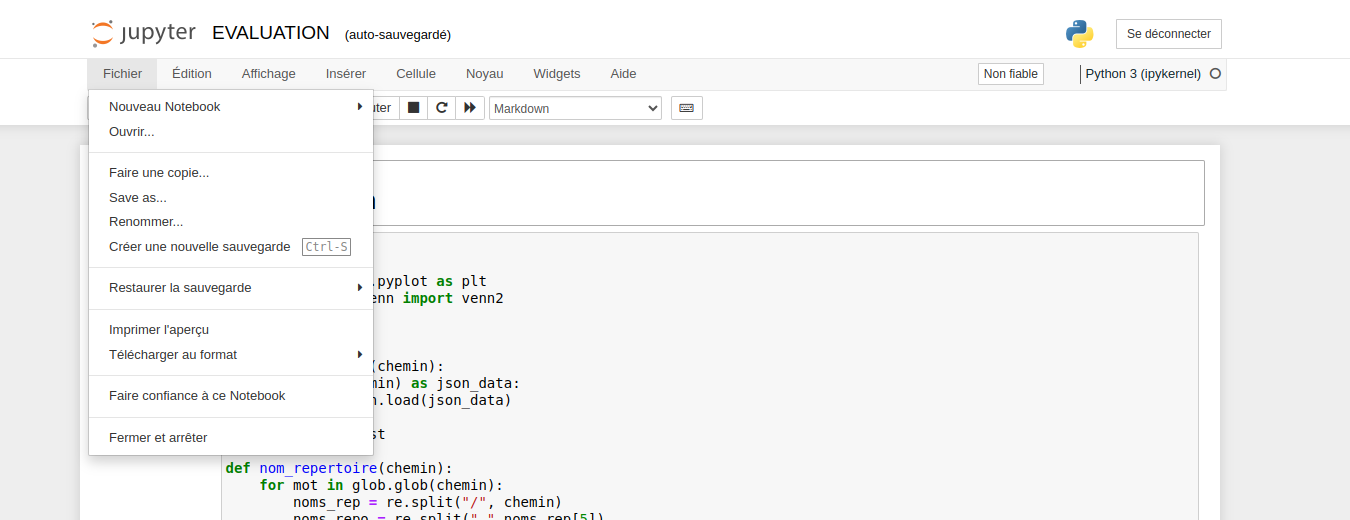
\includegraphics[width=10cm]{images/ynpb_convert_py.png}
  \end{figure}
 
\end{frame}



%\begin{frame}
%%  \frametitle{}
%  
%\end{frame}



\section{Spyder un autre environnement }  

\begin{frame} \frametitle{L'Éditeur 1}
  \begin{figure}
  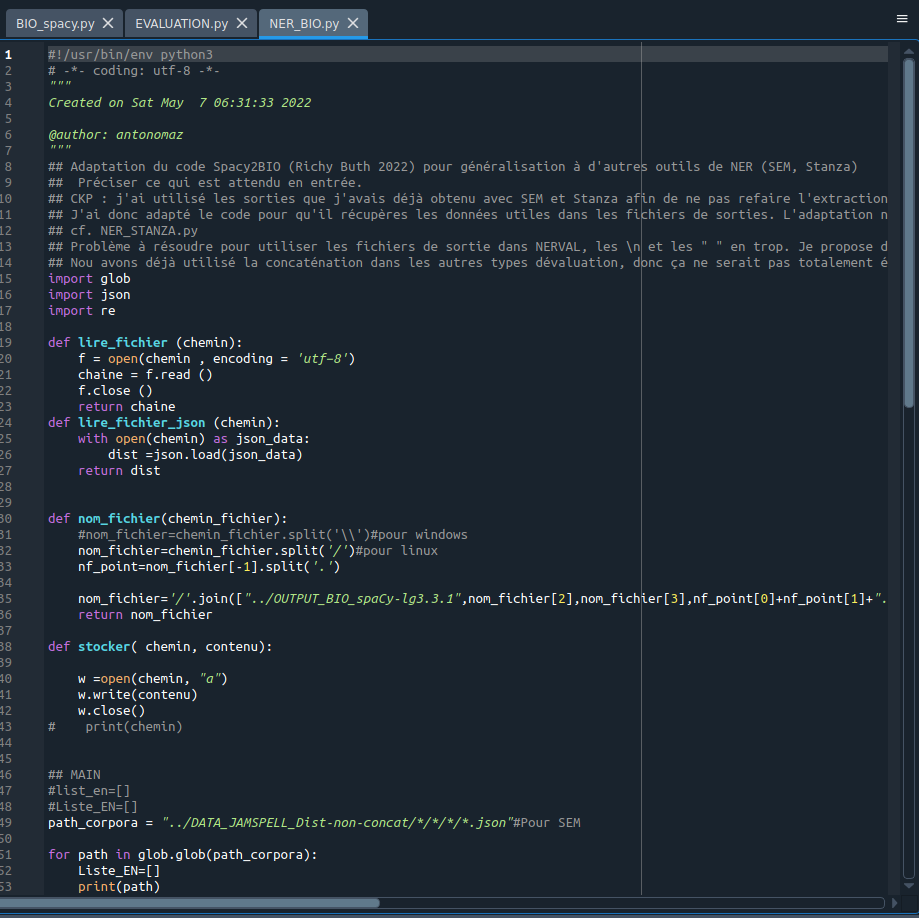
\includegraphics[width=7cm]{images/spyder_editor.png}
  \end{figure}
  
  \ding{220} +sieurs scripts peuvent être ouverts en même temps
\end{frame}

\begin{frame} \frametitle{L'Éditeur 2}

  \begin{figure}
  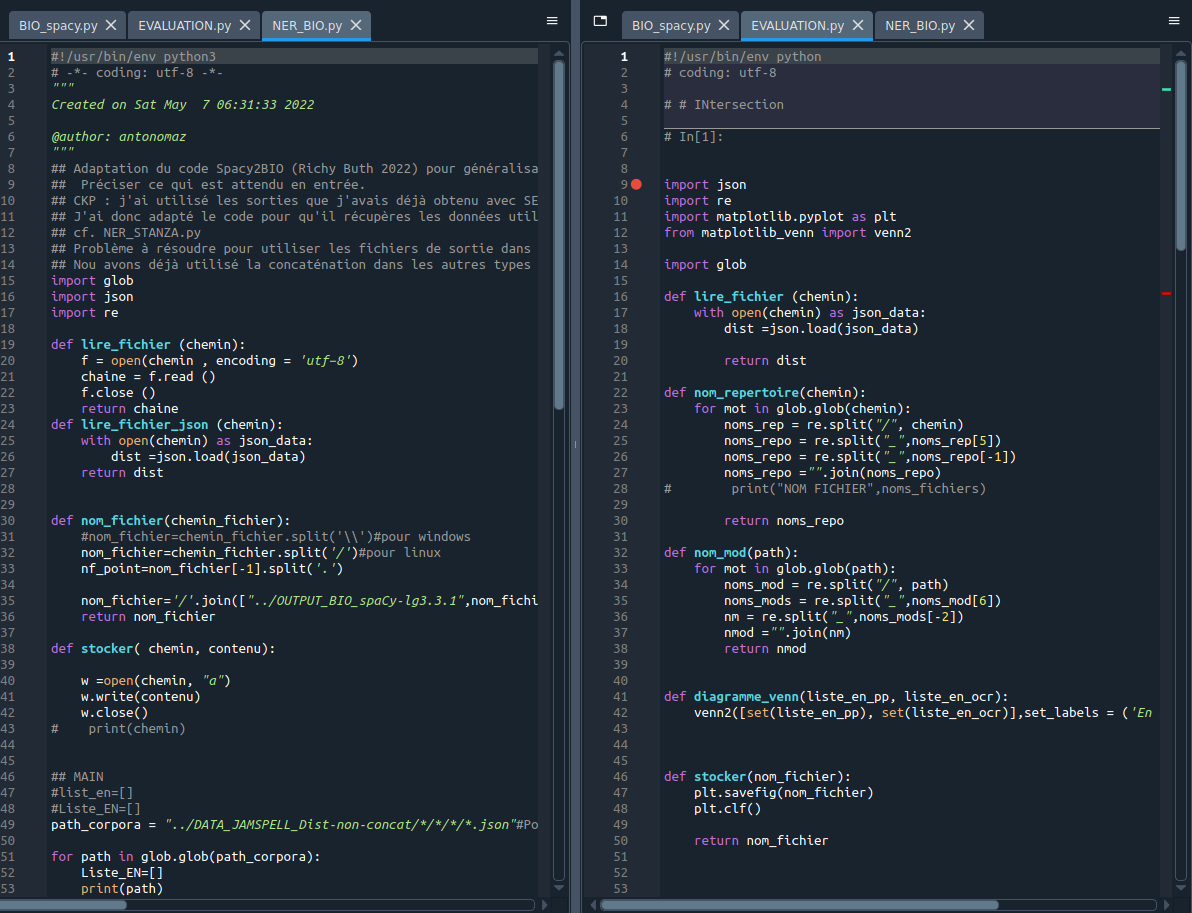
\includegraphics[width=7cm]{images/spyder_editor2.png}
  \end{figure}
  
  \ding{220} +sieurs scripts peuvent être ouverts côte à côte, ou l'un au dessus de l'autre.\\
  \ding{220} Cliquer sur
  \vspace{-0.3cm} 
  \begin{figure}
  
\includegraphics[width=0.5cm]{images/spyder_param.png}
  \end{figure} 
  \vspace{-0.3cm}
  et sélectionner \textit{split horizontally} ou \textit{split vertically}
\end{frame}

\begin{frame}  \frametitle{La console}
  \begin{figure}
  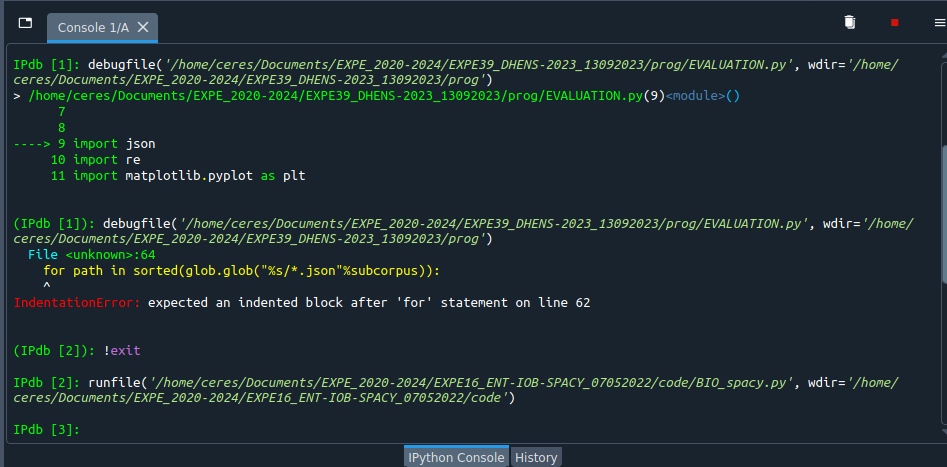
\includegraphics[width=10cm]{images/spyder_console.png}
  \end{figure}
  \ding{220} des lignes de codes peuvent être lancées depuis la console\\
  \ding{220} Les messages d'erreurs s'affichent dans la console \ding{219} Débogage\\
  \ding{220} Carré rouge en haut à droite de la console  == ordinateur calcul
\end{frame}

\begin{frame}
  \frametitle{Situer son script sur sa machine}
  \begin{figure}
  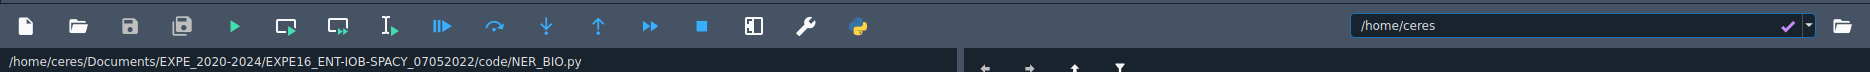
\includegraphics[width=15cm]{images/spyder_chemin.png}
  \end{figure}
  \ding{220} Haut droite, fil d'Ariane : Indique où votre script est rangé sur la machine\\
  \ding{220} Haut gauche : permet de changer de dossier racine, d'explorer l'arborescence de votre machine
\end{frame}

\begin{frame}
  \frametitle{Renseignements sur l'environnement}
  \begin{figure}
  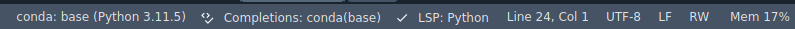
\includegraphics[width=10cm]{images/spyder_infos.png}
  \end{figure}
\end{frame}

\begin{frame}  
\frametitle{L'explorateur de variable}
\begin{figure}
  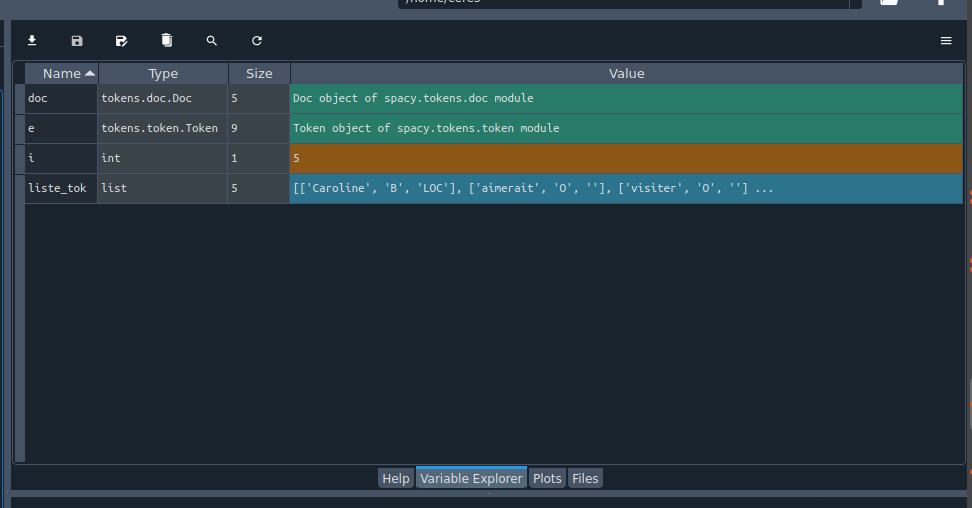
\includegraphics[width=10cm]{images/spyder_explo_variable.png}
  \end{figure}
\end{frame}

\begin{frame}
  \frametitle{Sélectionner un fichier}
  \begin{figure}
  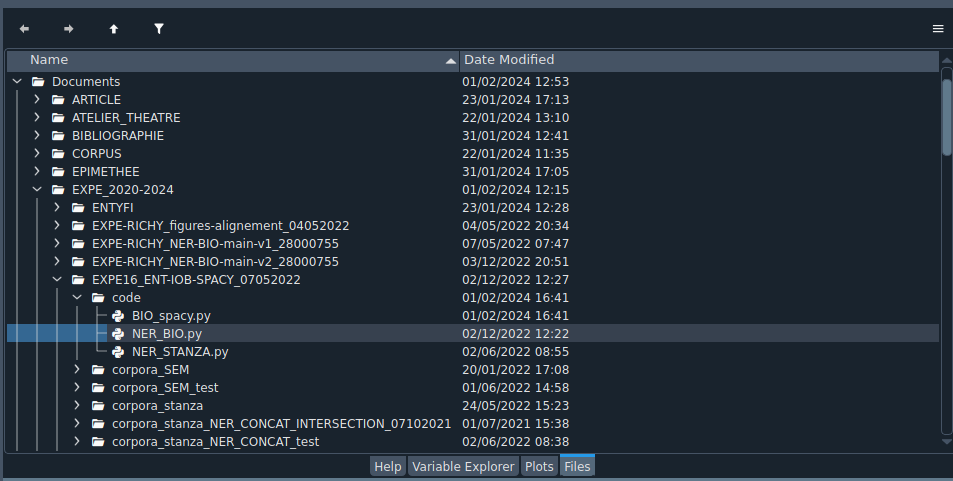
\includegraphics[width=10cm]{images/spyder_Files.png}
  \end{figure}
  \end{frame}

\begin{frame}
  \frametitle{Historique}
  \begin{figure}
  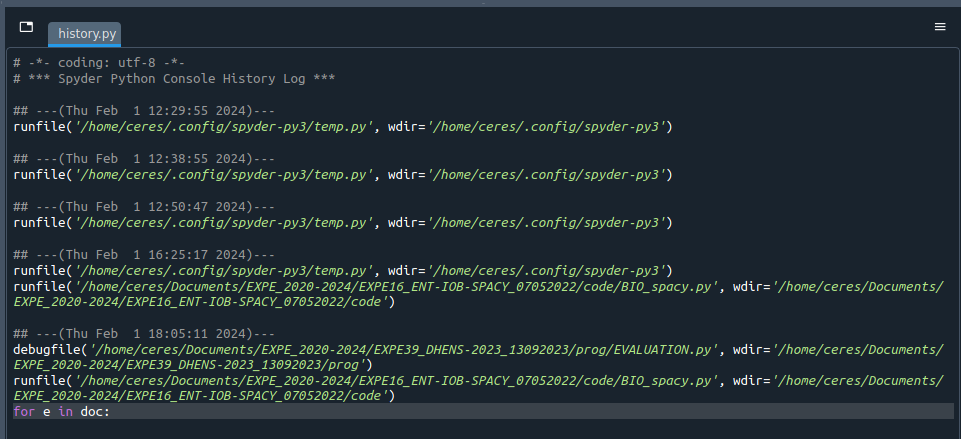
\includegraphics[width=10cm]{images/spyder_hystory}
	\end{figure}  
  \end{frame}
  
\begin{frame}
  \frametitle{Débogage base}
  \begin{figure}
  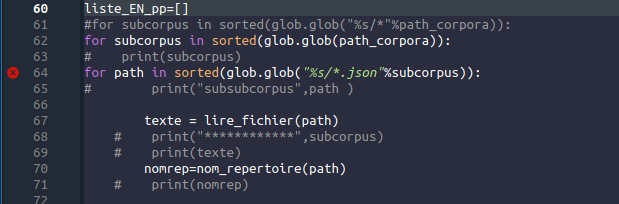
\includegraphics[width=10cm]{images/spyder_signal_erreur.png}
	\end{figure}  
  \end{frame}
  
\section{Listes, set et match !}

\begin{frame}
  \frametitle{Petit point sur les listes}
  Une liste est une structure de données permettant d'accéder
à un objet par son index.


Pour illustrer , supposons qu'une liste représente une rue.
Chaque habitant vit dans une maison avec un numéro.
Ce numéro est l'index de la liste grâce auquel on peut accéder
à l'habitant .


Syntaxe :
\begin{itemize}
\item* liste =[] :définition d'une liste vide
\item* liste =["Annie" , "Paul"] :défnition avec quelques éléments
\item* liste [0] vaut "Annie" , liste[1] vaut "Paul".
\end{itemize}



\end{frame}
\begin{frame}
%  \frametitle{}
  
\end{frame}
\begin{frame}
%  \frametitle{}
  
\end{frame}\begin{frame}
%  \frametitle{}
  
\end{frame}






